% Created by tikzDevice version 0.7.0 on 2015-01-10 18:42:07
% !TEX encoding = UTF-8 Unicode
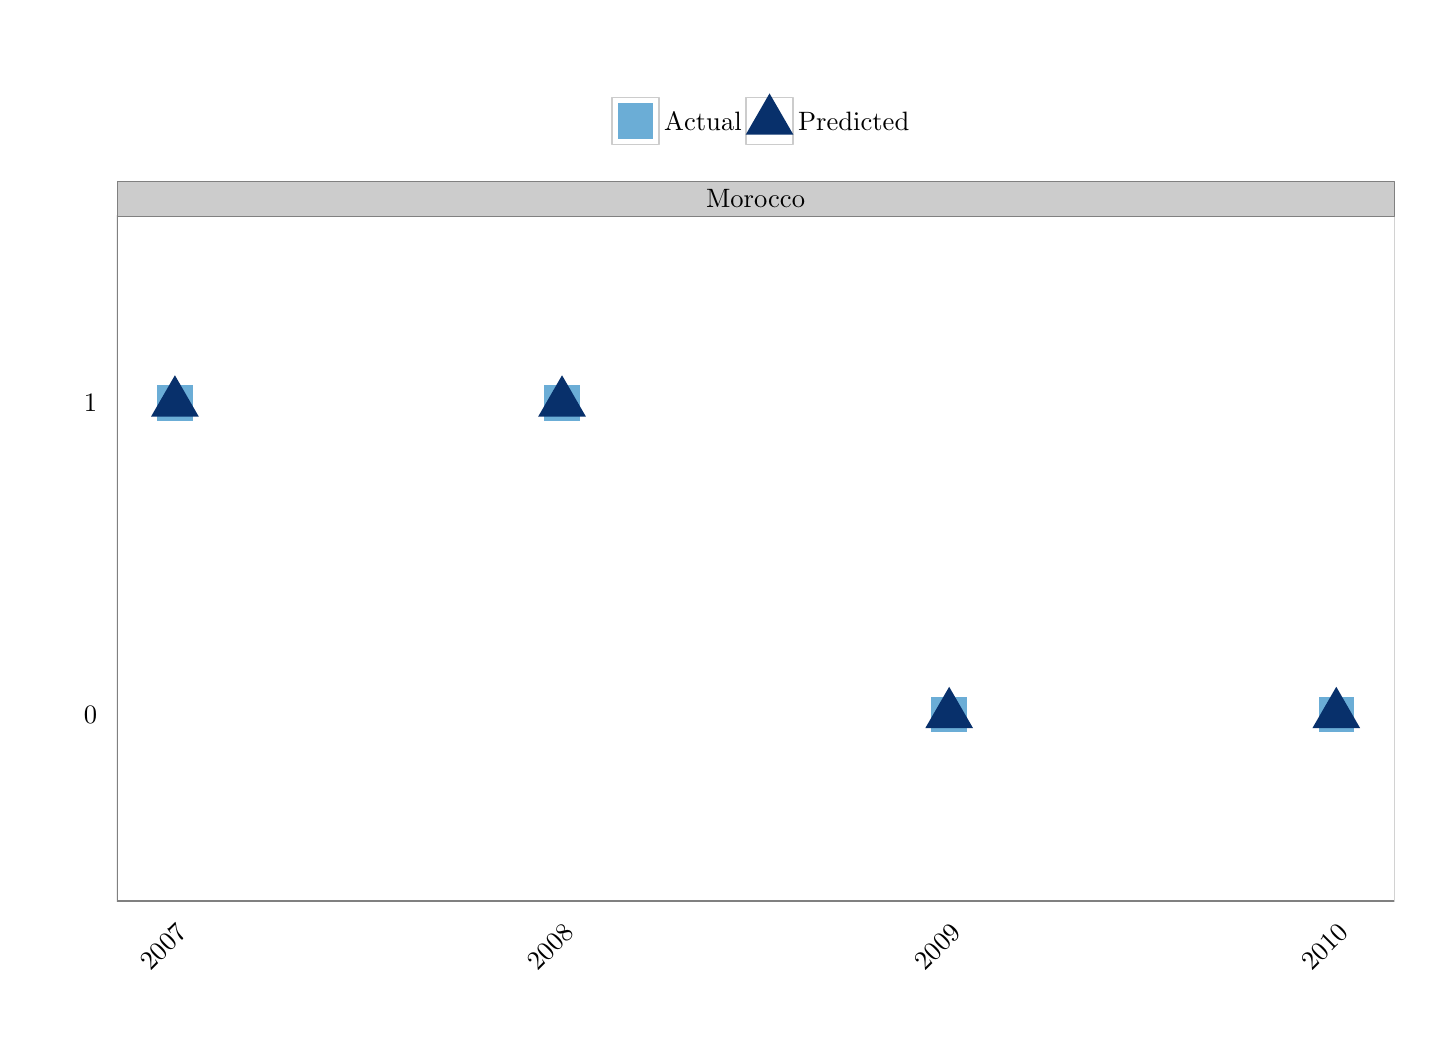
\begin{tikzpicture}[x=1pt,y=1pt]
\definecolor[named]{fillColor}{rgb}{1.00,1.00,1.00}
\path[use as bounding box,fill=fillColor,fill opacity=0.00] (0,0) rectangle (505.89,361.35);
\begin{scope}
\path[clip] (  0.00,  0.00) rectangle (505.89,361.35);
\definecolor[named]{drawColor}{rgb}{1.00,1.00,1.00}
\definecolor[named]{fillColor}{rgb}{1.00,1.00,1.00}

\path[draw=drawColor,line width= 0.6pt,line join=round,line cap=round,fill=fillColor] (  0.00,  0.00) rectangle (505.89,361.35);
\end{scope}
\begin{scope}
\path[clip] ( 32.22, 45.67) rectangle (493.85,293.33);
\definecolor[named]{fillColor}{rgb}{1.00,1.00,1.00}

\path[fill=fillColor] ( 32.22, 45.67) rectangle (493.85,293.33);
\definecolor[named]{fillColor}{rgb}{0.42,0.68,0.84}

\path[fill=fillColor] (466.46,106.81) --
	(479.26,106.81) --
	(479.26,119.62) --
	(466.46,119.62) --
	cycle;

\path[fill=fillColor] (326.57,106.81) --
	(339.38,106.81) --
	(339.38,119.62) --
	(326.57,119.62) --
	cycle;

\path[fill=fillColor] (186.69,219.38) --
	(199.49,219.38) --
	(199.49,232.19) --
	(186.69,232.19) --
	cycle;

\path[fill=fillColor] ( 46.80,219.38) --
	( 59.61,219.38) --
	( 59.61,232.19) --
	( 46.80,232.19) --
	cycle;
\definecolor[named]{fillColor}{rgb}{0.03,0.19,0.42}

\path[fill=fillColor] (472.86,123.17) --
	(481.48,108.24) --
	(464.24,108.24) --
	cycle;

\path[fill=fillColor] (332.98,123.17) --
	(341.60,108.24) --
	(324.35,108.24) --
	cycle;

\path[fill=fillColor] (193.09,235.74) --
	(201.71,220.81) --
	(184.47,220.81) --
	cycle;

\path[fill=fillColor] ( 53.20,235.74) --
	( 61.83,220.81) --
	( 44.58,220.81) --
	cycle;
\definecolor[named]{drawColor}{rgb}{0.50,0.50,0.50}

\path[draw=drawColor,line width= 0.6pt,line join=round,line cap=round] ( 32.22, 45.67) rectangle (493.85,293.33);
\end{scope}
\begin{scope}
\path[clip] (  0.00,  0.00) rectangle (505.89,361.35);
\definecolor[named]{drawColor}{rgb}{0.50,0.50,0.50}
\definecolor[named]{fillColor}{rgb}{0.80,0.80,0.80}

\path[draw=drawColor,line width= 0.2pt,line join=round,line cap=round,fill=fillColor] ( 32.22,293.33) rectangle (493.85,305.96);
\definecolor[named]{drawColor}{rgb}{0.00,0.00,0.00}

\node[text=drawColor,anchor=base,inner sep=0pt, outer sep=0pt, scale=  0.96] at (263.03,296.34) {Morocco};
\end{scope}
\begin{scope}
\path[clip] (  0.00,  0.00) rectangle (505.89,361.35);
\definecolor[named]{drawColor}{rgb}{0.00,0.00,0.00}

\node[text=drawColor,anchor=base east,inner sep=0pt, outer sep=0pt, scale=  0.96] at ( 25.11,109.91) {0};

\node[text=drawColor,anchor=base east,inner sep=0pt, outer sep=0pt, scale=  0.96] at ( 25.11,222.48) {1};
\end{scope}
\begin{scope}
\path[clip] (  0.00,  0.00) rectangle (505.89,361.35);
\definecolor[named]{drawColor}{rgb}{0.00,0.00,0.00}

\node[text=drawColor,rotate= 45.00,anchor=base east,inner sep=0pt, outer sep=0pt, scale=  0.96] at ( 57.88, 33.88) {2007};

\node[text=drawColor,rotate= 45.00,anchor=base east,inner sep=0pt, outer sep=0pt, scale=  0.96] at (197.77, 33.88) {2008};

\node[text=drawColor,rotate= 45.00,anchor=base east,inner sep=0pt, outer sep=0pt, scale=  0.96] at (337.65, 33.88) {2009};

\node[text=drawColor,rotate= 45.00,anchor=base east,inner sep=0pt, outer sep=0pt, scale=  0.96] at (477.54, 33.88) {2010};
\end{scope}
\begin{scope}
\path[clip] (  0.00,  0.00) rectangle (505.89,361.35);
\definecolor[named]{fillColor}{rgb}{1.00,1.00,1.00}

\path[fill=fillColor] (203.24,314.83) rectangle (322.83,340.44);
\end{scope}
\begin{scope}
\path[clip] (  0.00,  0.00) rectangle (505.89,361.35);
\definecolor[named]{drawColor}{rgb}{0.80,0.80,0.80}
\definecolor[named]{fillColor}{rgb}{1.00,1.00,1.00}

\path[draw=drawColor,line width= 0.6pt,line join=round,line cap=round,fill=fillColor] (211.12,319.10) rectangle (228.19,336.17);
\end{scope}
\begin{scope}
\path[clip] (  0.00,  0.00) rectangle (505.89,361.35);
\definecolor[named]{fillColor}{rgb}{0.42,0.68,0.84}

\path[fill=fillColor] (213.25,321.23) --
	(226.06,321.23) --
	(226.06,334.04) --
	(213.25,334.04) --
	cycle;
\end{scope}
\begin{scope}
\path[clip] (  0.00,  0.00) rectangle (505.89,361.35);
\definecolor[named]{drawColor}{rgb}{0.80,0.80,0.80}
\definecolor[named]{fillColor}{rgb}{1.00,1.00,1.00}

\path[draw=drawColor,line width= 0.6pt,line join=round,line cap=round,fill=fillColor] (259.53,319.10) rectangle (276.60,336.17);
\end{scope}
\begin{scope}
\path[clip] (  0.00,  0.00) rectangle (505.89,361.35);
\definecolor[named]{fillColor}{rgb}{0.03,0.19,0.42}

\path[fill=fillColor] (268.07,337.59) --
	(276.69,322.66) --
	(259.45,322.66) --
	cycle;
\end{scope}
\begin{scope}
\path[clip] (  0.00,  0.00) rectangle (505.89,361.35);
\definecolor[named]{drawColor}{rgb}{0.00,0.00,0.00}

\node[text=drawColor,anchor=base west,inner sep=0pt, outer sep=0pt, scale=  0.96] at (230.00,324.33) {Actual};
\end{scope}
\begin{scope}
\path[clip] (  0.00,  0.00) rectangle (505.89,361.35);
\definecolor[named]{drawColor}{rgb}{0.00,0.00,0.00}

\node[text=drawColor,anchor=base west,inner sep=0pt, outer sep=0pt, scale=  0.96] at (278.41,324.33) {Predicted};
\end{scope}
\end{tikzpicture}
